
\subsection{A critique of SHAP}

While SHAP has very strong theoretical foundations and its implementation is impressive, there are several issues with the approach that should be discussed.  First, we cannot agree with the formal SHAP definition of feature importance for the simple reason that SHAP measures $x_j$ impact as the magnitude of the deviations $x_j$ causes from the mean model prediction, $\overline{y}$, rather than deviations from $y=0$.   For example, given equation $y=x_1^2 + x_2 + 100$ from \figref{fig:quad-area}, the effect of $x_1$ on $y$ is clearly $x_1^2$ (whose impact is the area of the orange region), not $|\overline{y} - x_1^2|$, as defined by SHAP (grey region area). 

\begin{figure}[htbp]
\begin{center}
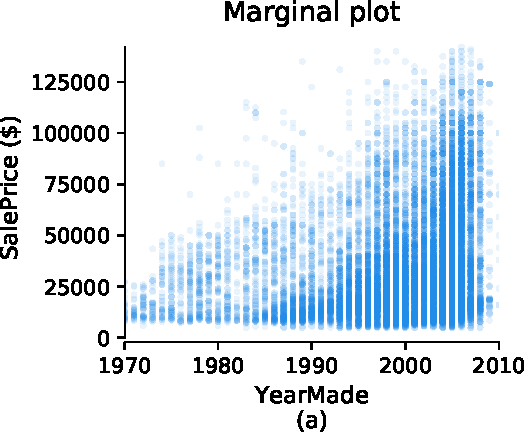
\includegraphics[scale=0.5]{images/bulldozer-YearMade-marginal.pdf}~~
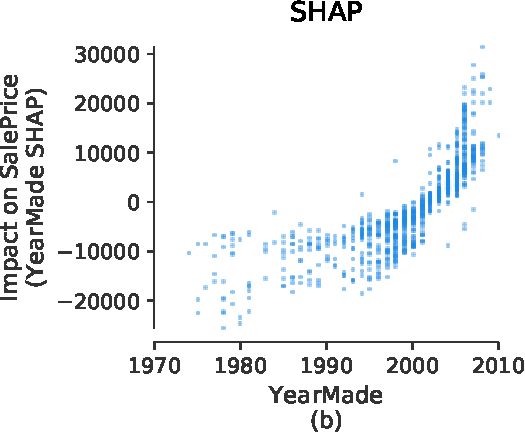
\includegraphics[scale=0.5]{images/bulldozer-YearMade-shap.pdf}~~
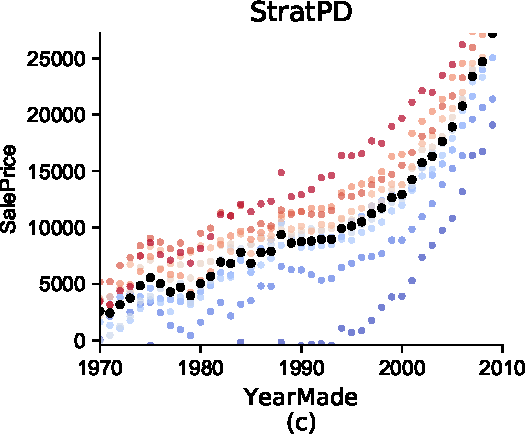
\includegraphics[scale=0.5]{images/bulldozer-YearMade-stratpd.pdf}
\caption{\small (a) Marginal plot of bulldozer {\tt YearMade} versus {\tt SalePrice} using subsample of 20k observations, (b) partial dependence drawn by SHAP interrogating an RF with 40 trees and explaining 1000 observations with 100 observations as background data, (c) \spd{} partial dependence.}
\label{fig:shap-stratpd-YearMade}
\end{center}
\end{figure}

Second, while the formal SHAP definition does not assume feature independence, the SHAP implementation does so for the specific purpose of simulating models trained on feature subsets. The SHAP definition approximates $\hat{f}_S(x_S)$ with $\Ex[\hat{f}(x_{S},{\bf X}_{\bar{S}}) | {\bf X}_S = x_S]$, but SHAP's implementation approximates $\hat{f}_S(x_S)$ with $\Ex[\hat{f}(x_{S},{\bf X}_{\bar{S}})]$, which requires feature independence for accuracy. \cite{janzing2019feature} argues that ``{\em unconditional} [as implemented] rather than {\em conditional} [as defined] expectations provide the right notion of dropping features.'' In practice, however, we have observed several instances of questionable SHAP partial dependence curves for features important to the model.  \figref{fig:shap-stratpd-YearMade} gives one such example, comparing (a) the marginal plot of  bulldozer {\tt YearMade} to {\tt SalePrice}, (b) SHAP partial dependence of {\tt SalePrice} on {\tt YearMade}, and (c) \spd{}'s curve. The SHAP plot does not show the expected relationship, that of decreased value for older bulldozers. One reasonable possibility is that other features are bleeding in, biasing the effect of {\tt YearMade}.

\begin{figure}[htbp]
\begin{center}
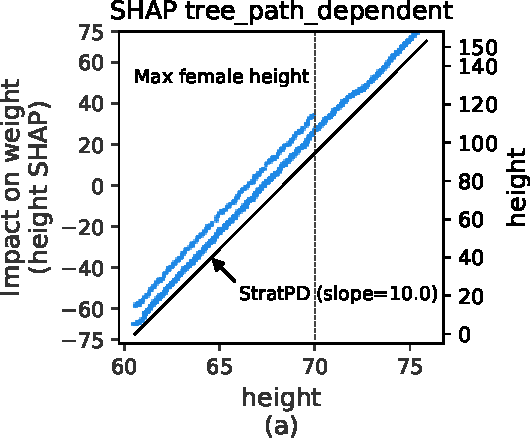
\includegraphics[scale=0.5]{images/weight-shap-tree_path_dependent.pdf}~~
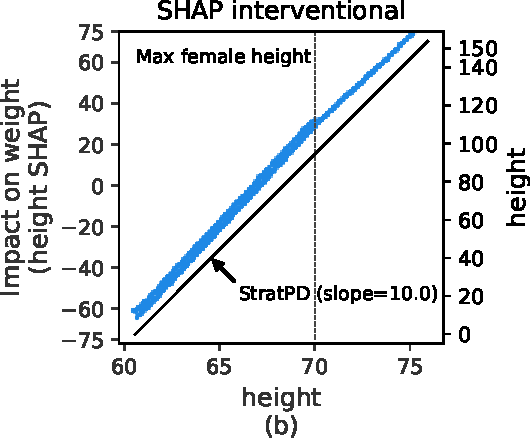
\includegraphics[scale=0.5]{images/weight-shap-interventional.pdf}
\caption{\small SHAP partial dependence plots of response body weight on feature {\tt height} using 2000 synthetic observations from Equation \eqref{eq:weight}. SHAP interrogated an RF with 40 trees and explained all 2000 samples; the interventional case used 100 observations as background data. \todo{just ref paper \#1}}
\label{fig:shap-weight}
\end{center}
\end{figure}


To explore the ability of SHAP to disentangle codependent features, we tested the SHAP implementation on a synthetic body weight data set with codependent {\tt\small sex}/{\tt\small pregnant}/{\tt\small height} features (Equation (7) from \citealt{stratpd}):

\begin{equation}\label{eq:weight}
y_{weight}  = 120 + 10(x_{height} - min(x_{height})) + 70x_{pregnant} - 1.5x_{education}
\end{equation}

\noindent with 50/50 male/female, half of the women are pregnant, and women gain an exaggerated 70 pounds to make the bias more prominent. \figref{fig:shap-weight}(a) illustrates the SHAP ``tree path dependent mode'' partial dependence between {\tt height} and response {\tt weight} and (b) shows that the interventional mode SHAP curve is better but still biased by codependent features.  The exact partial dependence relationship between {\tt height} and {\tt weight} should be a line with slope 10, which is what \spd{} computes and draws on top of the SHAP plots (using the righthand scale) in \figref{fig:shap-weight}; see \citet{stratpd} for more details.

This bias arises because the marginal expectation $\Ex[\hat{f}(x_{S},{\bf X}_{\bar{S}})]$ effectively replaces the $S$ features in all $\bf X$ records with $x_S$, which potentially conjures up nonsensical records, or at least records not in $\hat{f}$'s training set.  In this case, SHAP asks $\hat{f}$ to compute the body weight of pregnant males \todo{wrong. fix}. From a mathematical perspective, the bias is clear because $\Ex[\hat{f}(x_{S},{\bf X}_{\bar{S}})]$ is equivalent to $FPD_S(x)$ that is known to be biased by codependent features. (Equation 53 in \citealt{PDP} gives a summation equivalent to $\Ex[\hat{f}(x_{S},{\bf X}_{\bar{S}})]$).  

\begin{figure}[htbp]
\begin{center}
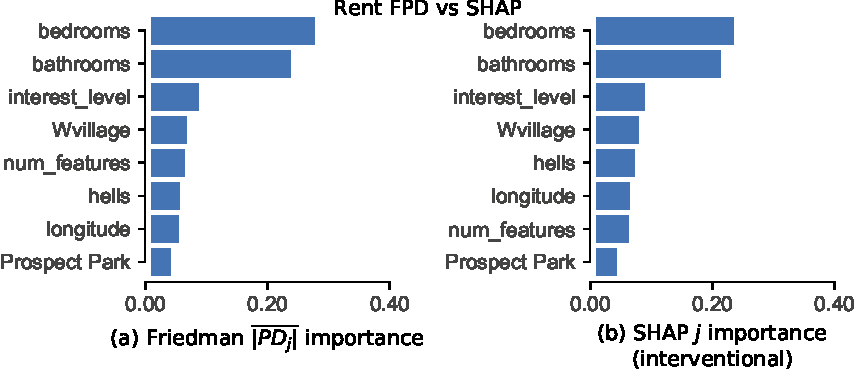
\includegraphics[scale=0.53]{images/rent-pdp-vs-shap.pdf}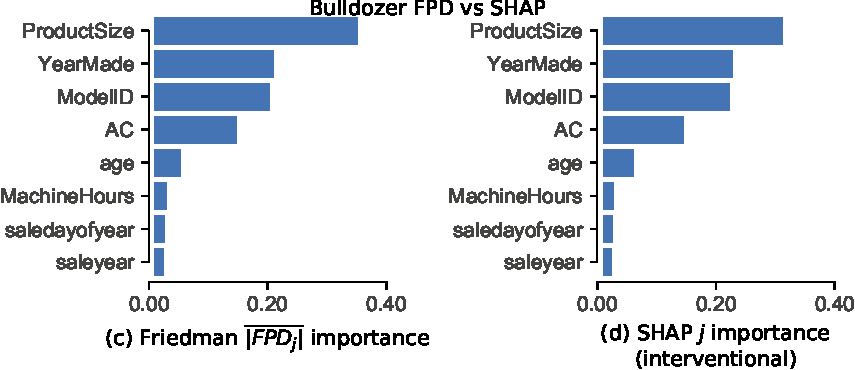
\includegraphics[scale=0.53]{images/bulldozer-pdp-vs-shap.pdf}
\caption[short]{\small  Feature importance ranking of top 8 for rent and bulldozer data sets demonstrating similarity between average magnitude of Friedman's partial dependence curves, (a) \& (c), and average magnitude of SHAP values, (b) \& (d). 20,000 training records and 300 records to explain. RF with 40 trees; Rent $R^2 = 0.82$, bulldozer $R^2 = 0.86$.}
\label{fig:fpd_imp}
\end{center}
\end{figure}

If the individual $\hat{f}(x_{S \texttt{\char`\\} \{j\}}) - \hat{f}(x_{S})$ contributions are known to be biased, measuring the effect of many $S$ permutations is likely unproductive. That begs the question of whether a one-off FPD curve would be just as effective as a SHAP implementation that  simulates feature dropping with $\Ex[\hat{f}(x_{S},{\bf X}_{\bar{S}})]$.  \figref{fig:fpd_imp} compares feature importances derived from FPD curves and SHAP values for two real data sets, rent and bulldozer. The rank and magnitude of the feature importances are extremely similar between the techniques for all $p$ features (top 8 shown here). At least for these examples, the complex machinery of SHAP is unnecessary because FPD gets virtually the same answer.

Our final concern is that SHAP effectively limits the user's choice of model to those with model-type-dependent implementations, such as {\tt\small TreeExplainer}, for efficiency reasons. For example, SHAP applied to a support vector machine (without a model-specific optimization) trained on Boston's 506 records takes 13 minutes to explain the same 506 records.  Large data sets also pose problems even for the model-type-dependent optimizations. SHAP applied to a modest 50-tree random forest trained on the 1.2M record ``League of legends'' data set \citep{lol} takes 25 minutes to explain a sample of size 1000.


\appendix

\section{Proof relating SHAP values and partial dependence curves}

The shapley regression values for features $F=\{1,..,p\}$ per \cite{shap} are as follows  using model $\hat{f}$.

\[
\phi_j(\hat{f},x) = \sum_{S \subseteq F \texttt{\char`\\} \{j\}}\
\frac{|S|!(|F|-|S|-1)!}{|F|!}\
 [ \hat{f}_{S \cup \{j\}}(x_{S \cup \{j\}}) - \hat{f}_S(x_S) ]
\]

\noindent In this section, we prove \thmref{thm}: $\Ex[ \phi_j(\hat{f},x) | {\bf X}_j = z] = FPD_j(x) - \bar{y}$.

\begin{proof}
{\em Part 1: } Show $\phi_j(\hat{f},x)$ is the difference between $\hat{f}(x)$ and the FPD curve, as defined by Friedman, for features $F \texttt{\char`\\} \{j\}$ (all features except $j$). For independent features, we can choose any single subset $S \subseteq F \texttt{\char`\\} \{j\}$ to measure the impact of feature $j$, therefore, we choose $S = F \texttt{\char`\\} \{j\}$.  With a single subset, the summation and weight term drop out:

\[
\phi_j(\hat{f},x) = \hat{f}_{S \cup \{j\}}(x_{S \cup \{j\}}) - \hat{f}_S(x_S)
\]

\noindent SHAP's implementation approximates $\hat{f}$ trained on just $S$ features, $\hat{f}_S(x_S)$, with $\Ex[\hat{f}(x_{S},{\bf X}_{\bar{S}})]$ by assuming independent features.  (SHAP unit testing support code in {\tt\small bruteforce.py}\footnote{\tt https://github.com/slundberg/shap/blob/master/shap/explainers/bruteforce.py} assumes independent features to approximate $\hat{f}_S(x_S)$.)

\[
\phi_j(\hat{f},x) = \
 \Ex[\hat{f}(x_{S \cup \{j\}},{\bf X}_{\overline{S \cup \{j\}}})] - \Ex[\hat{f}(x_{S},{\bf X}_{\bar{S}})]
\]

\noindent  That expectation expands to summation:

\[
\Ex[\hat{f}(x_{S},{\bf X}_{\bar{S}})] = \
    \frac{1}{n} \sum_{i=1}^n \hat{f}(x_S, x_{\bar{S}}^{(i)})
\]

\noindent But, that is equivalent to the approximation of $S$'s partial dependence curve (Equation 53 in \citealt{PDP}), giving:

\[
\begin{split}
\phi_j(\hat{f},x) & = \text{\it FPD}_{S \cup \{j\}}(x) - \text{\it FPD}_{S}(x)\\
 & = \text{\it FPD}_{F}(x) - \text{\it FPD}_{F \texttt{\char`\\} \{j\}}(x)
\end{split}
\]

\cut{
$\phi_j$ is, therefore, the difference between points on two partial dependence curves, one curve derived using $F$, which is just $\hat{f}(x)$, and one derived from $F \texttt{\char`\\} \{j\}$. 
}

\noindent  Because $\text{\it FPD}_{F}(x) = \hat{f}_F(x_F) = \hat{f}(x)$, the equation simplifies to the difference between $\hat{f}(x)$ and the marginal effect of $j$ at point $x$:

\[
\phi_j(\hat{f},x) = \hat{f}(x) - \text{\it FPD}_{F \texttt{\char`\\} \{j\}}(x)
\]

\noindent {\em Part 2}. Show that the expected SHAP value at a specific $x_j=z$ value is a point on the mean-centered FPD curve:


\[
\Ex[ \phi_j(\hat{f},x) | {\bf X}_j = z] = \text{\it FPD}_j(x) - \bar{y}
\]

\noindent Take the expected value of $\phi_j(\hat{f},x)$ conditioned on each instance in $\bf X$ using value $z$ for feature $j$:

\[
\Ex[ \phi_j(\hat{f},x) | {\bf X}_j = z ] = \Ex [\hat{f}(x) | {\bf X}_j = z ] - \Ex [ \text{\it FPD}_{F \texttt{\char`\\} \{j\}}(x) | {\bf X}_j = z ]
\]

\noindent  Because of independence, $\Ex [\hat{f}(x) | {\bf X}_j = z ] = \Ex [\hat{f}(x_j,x_{\bar{j}}) ]$, which is the definition of $FPD_j(x)$:

\[
\Ex[ \phi_j(\hat{f},x) | {\bf X}_j = z ] = FPD_j(x) - \Ex [ \text{\it FPD}_{F \texttt{\char`\\} \{j\}}(x) | {\bf X}_j = z ]
\]

\noindent $\text{\it FPD}_{F \texttt{\char`\\} \{j\}}(x)$  fixes $F \texttt{\char`\\} \{j\}$ and the conditional ${\bf X}_j = z$ fixes $j$, yielding 

\[
\Ex[ \phi_j(\hat{f},x) | {\bf X}_j = z ] = FPD_j(x) - \Ex_{\bf X} [ \text{\it FPD}_{F}(x) ]
\]

\noindent Since, $\text{\it FPD}_{F}(x) = \hat{f}(x)$:

\[
\begin{split}
\Ex[ \phi_j(\hat{f},x) | {\bf X}_j = z ] &= FPD_j(x) - \Ex_{\bf X} [ \hat{f}(x) ]\\
 & = FPD_j(x) - \bar{y}
\end{split}
\]

\noindent which completes the proof.

\end{proof}


